\section{Equality in the two-tree bound and quartic growth}
\label{sec:two-tree-equality-new}

Write $b=|\partial G|$, $i=|V(G)\setminus\partial G|$, and
$e=b-i-4=2b-|V(G)|-4$.  This section strengthens the sharp two-tree
bound $b\ge\lceil n/2\rceil+2$ for $n\ge6$.  Its most pronounced
consequence is a difference between the two parities.

\begin{theorem}[Complete equality grammars and growth]
Let $a_n$ be the number of isomorphism classes of two-trees on $n$ vertices
attaining $b=\lceil n/2\rceil+2$.
Then $a_6=2$ and $a_n=3$ for every even $n\ge8$.  At odd orders,
\[
 a_n\sim n^4/192.
\]
More explicitly, for every odd $n\ge19$,
\[
 a_n\ge \frac18\binom{(n-19)/2+4}{4}.
\]
All odd extremizers with noncomplete degree-two-pruned core are given by
an explicit finite grammar with $27$ states, $83$ productions, and $194$
terminal choices.  Exactly two additional complete-core examples occur,
both at order seven.  Every extremizer, of either parity, has maximum
degree at most six.
\end{theorem}

The exact rational generating function and period-eight formula are
proved in the subsequent exact-enumeration section.  The argument
below retains a separate proof of the quartic growth order.

The finite grammar is a necessary-and-sufficient description at every
order, rather than a list inferred from an initial census.  Its
graph-theoretic semantics are proved below; independent integer
checkers regenerate the complete state closure and certify the
pruning.  The grammar data are in
\texttt{checks/extensions/two\_tree\_equality/}.

\subsection{A structural defect identity}

Use the injective assignment from degree-five interior vertices to
boundary vertices established in the sharp-bound proof.  Path links
are assigned their degree-three middle and fork links their
degree-four branch.  Let $f$ count fork assignments and let $U$ be the
unassigned boundary vertices.  The exact degree identity is
\begin{equation}
 2e+2=f+\sum_{x\in U}(\deg x-2)
       +\sum_{\substack{x\notin\partial G\\\deg x\ge7}}(\deg x-6).
 \label{eq:new-defect}
\end{equation}
All terms are nonnegative.

Delete all degree-two vertices and call the resulting graph $H$.
If $H$ is noncomplete, it is a two-tree.  Every degree-two vertex of
$H$ is boundary in $G$, by the pruning lemma.  It cannot be an assigned
path middle, because all three neighbors of such a middle have
original degree greater than two.  Each core ear therefore consumes
at least one distinct unit of \eqref{eq:new-defect}.  Since $H$ has at
least two ears, this gives
\begin{equation}
 \begin{aligned}
 \#\{x:\deg_Hx=2\}&\le 2e+2,\\
 \deg_Gx&\le2e+6 &&(x\notin\partial G),\\
 \deg_Gx&\le\max(4,2e+3) &&(x\in\partial G).
 \end{aligned}
 \label{eq:new-structure}
\end{equation}
For the last bound, an unassigned boundary core ear leaves one unit
for another core ear; an unassigned boundary non-ear leaves two.
Assigned boundary vertices have degree at most four.

The triangle--edge incidence graph of a two-tree is a bipartite tree.
Remove its edge-nodes of degree one.  For noncomplete $H$, the leaves
of the remaining tree correspond exactly to its ears.  Thus its total
branching excess is at most $2e$.

There are elementary complete-core exceptions.  If $H=K_2$, all
vertices are boundary and $n=e+4$.  If $H=K_3$, write $p,q,r$ for the
numbers of attached ears on its three edges.  At least two numbers
are positive.  A core vertex is interior exactly when its opposite
multiplicity is zero and both incident multiplicities are positive.
Consequently, three positive multiplicities give $n=e+4$ and
$p+q+r=e+1$, all boundary; exactly two positive multiplicities give
$n=e+6$ and $p+q=e+3$, with one interior vertex.  Retain only cases
with $n\ge6$.  At $e=0$ this gives $(p,q,r)=(1,2,0)$, and at $e=1$
it gives $(1,3,0)$ and $(2,2,0)$, up to permutation.

\subsection{Even equality: precisely three strips}

At $e=0$, both units of \eqref{eq:new-defect} are consumed by two core
ears, so the internal incidence tree of $H$ is a path.  All interior
degrees are five or six and all boundary degrees are at most four.

For $r\ge2$, start with a path $v_1,\ldots,v_r$ and independent
vertices $c_1,\ldots,c_r$.  Join $c_j$ to $v_j$ and every existing
path neighbor of $v_j$.  At either endpoint $v$, with corresponding
$c$, choose a cap:
\begin{itemize}
\item $P$: add $p$ on edge $vc$, then $q$ on edge $vp$;
\item $F$: add $p$ and $q$ separately on edge $vc$.
\end{itemize}
These give $PP(r),PF(r),FF(r)$, with $2r+4$ vertices.  The $r$ path
vertices are interior of degree five; all others are boundary.  Their
numbers of degree-four boundary vertices are respectively zero, one,
and two, so they are pairwise nonisomorphic.

For completeness, process the triangle path $H$ from one end.  For
each active endpoint record current degree and accumulated local
boundary requirement, and record the final triangle multiplicity of
the active edge.  The exact local formula is
\begin{equation}
 \beta(u)=R_u-\deg u,\qquad
 R_u=\max\{2+t_{uv},\ 2+t_{ua}+t_{ub}:
                   uab\text{ a triangle},\ t_{ab}\ge2\}.
 \label{eq:new-local}
\end{equation}
Here $t_{uv}$ is the number of triangles on edge $uv$.  Requirements
can be capped at seven.  Forget a boundary vertex of degree three or
four with weight $+1$, or an interior vertex of degree five or six
with weight $-1$; each added ear has weight $+1$.  Accepted weight is
exactly $b-i$.

The complete closure has $18$ states and $58$ ordinary parameterized
transitions.  Exact prefix and suffix potentials show that weight
four paths use only these four states and arcs:
\[
\begin{array}{c|c|c|c}
 &((d_u,R_u),(d_v,R_v),t)&\text{initial}&\text{terminal}\\ \hline
A&((2,5),(3,4),2)&2&2\\
B&((2,5),(4,4),2)&-&1\\
C&((2,5),(3,5),2)&-&2\\
D&((2,5),(4,5),2)&3&1
\end{array}
\]
\[
 A\longrightarrow B\ (+1),\quad B\longrightarrow C\ (-1),\quad
 C\longrightarrow D\ (+1),\quad D\longrightarrow C\ (-1).
\]
The initial and final choices give the $P,F$ caps.  More explicitly,
in state $C$ the active edge is $(c_j,v_j)$ of degrees $(2,3)$.
The step to $D$ adds $v_{j+1}$, forgets $c_j$ as a degree-three boundary
vertex, and retains $(v_{j+1},v_j)$ of degrees $(2,4)$.  The return
step adds $c_{j+1}$, forgets $v_j$ as a degree-five interior vertex,
and retains $(c_{j+1},v_{j+1})$.  Thus the cycle is exactly strip
extension.  The two order-six exceptions are the cones over the
five-vertex path and the five-vertex fork.  This proves the full even
classification.

\begin{figure}[htbp]
\centering
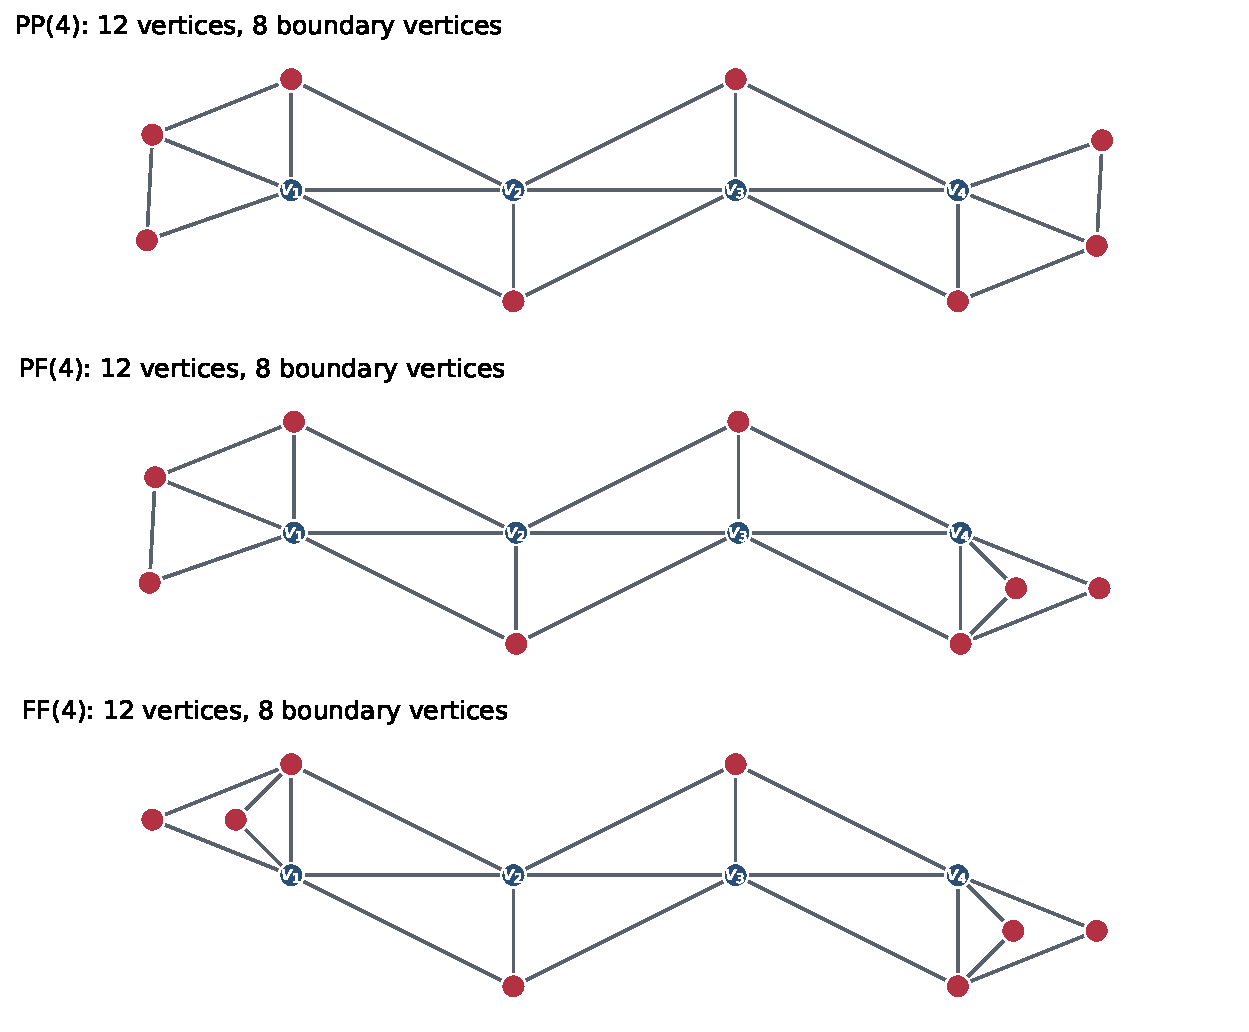
\includegraphics[width=.88\textwidth]{figures/even_extremal_families.pdf}
\caption{The three even extremal families at $r=4$. Blue vertices are the
four degree-five interior vertices; red vertices form the eight-point boundary.}
\end{figure}

\subsection{An exact rooted grammar at odd equality}

For $e=1$, \eqref{eq:new-structure} initially bounds interior degree
by eight, boundary degree by five, and core leaves by four.  A rooted
component has a pending root edge $uv$ and at least one outside core
triangle.  Its root ears are deferred.  If $k$ is the number of inside
core triangles on that edge, record at each endpoint a triple
$(d,A,B)$ whose requirement, at final root multiplicity $t\ge2$, is
\[
 \rho(t)=\max(A,B+t).
\]
The state is $(k;d_u,A_u,B_u;d_v,A_v,B_v)$, with endpoint triples
sorted.  Continuing degrees are at most seven; cap $A$ at nine and
$B$ at seven.  These caps preserve all decisions at final degree at
most eight.  A rooted component has one, two, or three leaves.

This information is sufficient: a forgotten vertex has every incident
edge closed.  Its only possible dependence on the pending root edge
is as the opposite edge of a triangle, whose active condition is
merely $t\ge2$ and is already fixed.  The two retained requirements
remain maxima of a constant and a constant plus $t$.

The operations are: an initial leaf triangle with ears on its closed
edges; adding one triangle and retaining a new root edge; joining
two components at a triangle; and identifying two pending root
edges.  In the last operation degrees add with subtraction of one,
because the root neighbor is counted twice, while $k,A,B$ combine by
addition, maximum, maximum, respectively.  In a triangle join, the
degree of the identified vertex is the sum of its child degrees
without subtraction.  All formulas follow directly from
\eqref{eq:new-local} and are given explicitly in the supplied note.
Final gluing identifies the two pending roots, adds any root ears,
and finalizes both endpoints.  Every forgotten vertex is required
to be boundary of degree three through five or interior of degree
five through eight.  Its sign, together with the ears, contributes
to component weight; the two pending roots are excluded.

Rooting the internal incidence tree at an internal edge yields two
components, each with at most three leaves.  Recursion into that
tree gives exactly the four operations.  This proves necessity;
the same interpretation and local formula prove sufficiency.
When the numerical root triples coincide, either physical ordering
is permitted: equal data do not imply a swapping automorphism.
No final productive equality state has such a tie.

The complete raw closure has $88,985,1153$ states with one, two,
three leaves, respectively.  It has nine initial, $126968$ binary,
and $6030$ unary productions.  Let $\mu(s)$ be the minimum component
weight.  The certified potentials satisfy, for every production,
\[
 \sum_j\mu(s_j)+w-\mu(s)\ge0.
\]
Rank-decreasing productivity witnesses attain every minimum.  A
minimum completed gluing is an actual graph and has weight at least
four.  Thus any accepted weight-five derivation has slack at most
one above its component minima.  Adding a slack coordinate $0$ or
$1$, retaining productive states, and tracing backwards from
weight-five terminal choices gives precisely $27$ states, $83$
productions, and $194$ terminal choices.  The two complete-core
exceptions at order seven finish the classification.

An independent verifier regenerates all raw rules and all $113830$
valid terminal gluings, checks $133007$ potential inequalities, and
checks the rank certificates and exact backward pruning.  A separate
program realizes all $4386$ productivity witnesses as actual graphs
and recomputes their full distance boundary scores by BFS.  Both
checks pass.  Every interior degree appearing in an accepted rule
or terminal choice is five or six.  This proves the claimed uniform
degree-six bound.

\subsection{Five strip parameters suffice}

The compact odd grammar has no triangle-join production.  Its pending
root multiplicities satisfy $k\le2$, and final root core multiplicity
is at most three.  Thus the internal core incidence tree branches
only at trivalent edge-nodes, with at most two branches.

Number the compact states from zero in the order in the data file.
The only cyclic strongly connected components of its unary part are
\[
 \{1,4\},\quad\{2,5\},\quad\{10,11\},\quad\{22,23\},
 \quad\{6\},\quad\{12\}.
\]
Each state has exactly one rule staying inside its cyclic component.
The two-step cycles insert a degree-five strip pair; the self-loops
insert a degree-six core vertex together with an ear.  Every complete
cycle has weight zero and adds exactly two vertices.

After contracting these components, the dependence graph is acyclic;
binary rules increase leaf count.  Consequently derivations consist
of finitely many templates, with one repetition parameter for each
cyclic component occurrence.  To count occurrences rather than just
topological core paths, assign to each contracted component $C$
\[
 M(C)=\mathbf1_{C\text{ cyclic}}+
 \max\Bigl\{\sum_j M(C_j):
    \text{a production enters }C\text{ from children outside }C\Bigr\}.
\]
The exact per-state vector is
\[
\begin{split}
(&0,1,3,0,1,3,2,0,1,2,4,4,3,3,0,2,\\
 &0,1,2,1,2,3,5,5,4,3,4).
\end{split}
\]
If the core branches, root at a trivalent edge-node, so the terminal
choice has $k_1+k_2=3$.  The maximum sum of these two state values is
five.  If the core is a path, root next to an end triangle: that side
is an initial leaf, with no repetition parameter, and the other side
has at most three.  Thus every odd extremizer has a finite-template
description with at most five nonnegative repetition parameters.
Each parameter adds two vertices, so at fixed order there are
$O(n^4)$ descriptions.  Ambiguity of descriptions can only reduce
the number of isomorphism classes.  This proves the upper bound.

\subsection{A matching five-parameter family}

Define a rooted arm $A(a)$, $a\ge0$, by taking a triangle $xyz$,
adding two ears on $xz$, adding $w$ on $yz$, and declaring the root
to be $(w,y)$, of degrees $(2,3)$.  Repeat $a$ times: on root
$(\ell,h)$ add $t$, then add $z'$ on $ht$, retaining root $(z',t)$.
This is compact state 1, of weight two and order $6+2a$.

Identify the low root endpoints and the high root endpoints of two
arms $A(a),A(b)$.  The resulting cherry $B(a,b)$ has root degrees
$(3,5)$, state 15, weight four, and order $10+2(a+b)$.
Starting with $B(c,d)$, add one vertex on its root edge and retain
the new vertex followed by the old low endpoint as root.  Its root
degrees are $(2,4)$, state 12, and weight three.  Repeat $r$ times:
add an ear and a continuing core vertex on this root edge, retaining
the new core vertex followed by the old low endpoint.  Each such
loop preserves state and weight and adds two vertices.

Finally identify this root crosswise with that of $B(a,b)$.  Both
final root endpoints have degree six and requirement six, so are
interior.  The resulting $F(a,b,c,d,r)$ satisfies
\[
 |V(F)|=19+2(a+b+c+d+r),\qquad b(F)-i(F)=4+3-2=5.
\]
It is therefore extremal for every nonnegative choice of parameters.

Its canonical degree-two-pruned core incidence tree has two trivalent
edge-nodes.  The four pendant paths contain $2+2a,2+2b,2+2c,2+2d$
triangle-nodes, in pairs at the two branches.  The path between the
branches contains $r+1$ triangle-nodes.  An isomorphism thus
determines $r$ and the unordered pair $\{\{a,b\},\{c,d\}\}$.  At
most eight ordered tuples can describe one isomorphism class.
For sum $S$, there are $\binom{S+4}{4}$ tuples, yielding the stated
lower bound.  Combined with the upper bound, this proves
$a_n=\Theta(n^4)$ through odd $n$.

The recovered incidence-tree lengths are graph invariants, as
shown above.  As a numerical check, all $792$
tuples of sum at most seven, reaching order 33, pass fresh BFS
boundary checks and exact parameter recovery.  The subsequent section
strengthens this result to an exact generating function and leading
coefficient by resolving all isomorphism identifications.

\subsection{Finite-state classification at every fixed excess}

\begin{theorem}[Effective fixed-excess grammar]
For each fixed integer $e\ge0$, the two-trees of order at least six
with $2b-n-4=e$ are generated by an effectively constructible finite
grammar, together with the explicit complete-core cases above.
Put $C=2e+6$, $L=2e+2$, and $K=(C-2)^2(C-1)$.  The grammar needs
at most
\[
 (e+1)(L-1)^2\frac{K(K+1)}2=O(e^9)
\]
states.
\end{theorem}

\begin{proof}
Use \eqref{eq:new-structure} and the same rooted requirements
$\max(A,B+t)$.  A continuing endpoint has degree in $[2,C-1]$;
cap $A$ at $C+1$ and $B$ at $C-1$.  Since $t\ge2$, both caps
preserve all boundary comparisons.  The endpoint triples thus
have $K$ possible numerical values.  The inside root multiplicity
and leaf count both lie in $[1,L-1]$.  Sorting the two triples gives
at most $(L-1)^2K(K+1)/2$ raw state/leaf pairs.  Ear multiplicities
are also bounded by degree.  The four operations and final gluing
remain exact, and cover every core of at most $L$ leaves.

Every reachable component weight is bounded below.  Indeed, fill its
pending root with one outside triangle and no root ears.  Previously
forgotten statuses are unchanged because root multiplicity remains
at least two.  The completed two-tree has weight at least four at
order at least six, and at least three at smaller orders.  Its two
former roots and new vertex contribute at most three.  Thus all
component weights are nonnegative, and state minima are attained
integers.  They can be computed by increasing leaf count: binary
joins use smaller counts and unary extensions give a finite
shortest-path problem without reachable negative cycles.

Reduced production costs are nonnegative.  Every minimum completed
gluing is an actual graph of weight at least four, so for target
$e+4$, each subcomponent's slack is in $[0,e]$.  Adjoining this
budget coordinate, retaining productive states, and accepting
exact total weight $e+4$ yields the claimed finite grammar and state
bound.  The complete-core cases have already been classified.
\end{proof}

This theorem does not assert polynomial unlabelled growth at every
fixed excess.  The deterministic cyclic structure required for the
quartic statement was certified specifically for $e=1$.

\paragraph{Formal verification scope.}
The Lean file \texttt{EvenEqualityAutomaton.lean} proves that every
accepted run, of arbitrary length, has weight at least four and
that every weight-four run uses only the four optimal transitions.
The odd finite grammar is also accompanied by a universal
derivation-weight and interior-degree certificate.  The
graph-to-state correspondence, core reduction, and counting
argument are ordinary mathematical proofs supported by independent
exact checkers; they are not claimed as end-to-end Lean
formalizations.
